
\documentclass[12pt]{article} 
\usepackage[margin=1in]{geometry} 
\usepackage{amsmath,amsthm,amssymb}
\usepackage{graphicx} %package to manage images
\graphicspath{ {images/} }

\newcommand{\N}{\mathbb{N}}
\newcommand{\Z}{\mathbb{Z}}
\newenvironment{definition}[2][Definition]{\begin{trivlist}
\item[\hskip \labelsep {\bfseries #1}\hskip \labelsep {\bfseries #2}]}{\end{trivlist}}
\newenvironment{lemma}[2][Lemma]{\begin{trivlist}
\item[\hskip \labelsep {\bfseries #1}\hskip \labelsep {\bfseries #2}]}{\end{trivlist}}
\newenvironment{exercise}[2][Exercise]{\begin{trivlist}
\item[\hskip \labelsep {\bfseries #1}\hskip \labelsep {\bfseries #2}]}{\end{trivlist}}
\newenvironment{problem}[2][Problem]{\begin{trivlist}
\item[\hskip \labelsep {\bfseries #1}\hskip \labelsep {\bfseries #2}]}{\end{trivlist}}
\newenvironment{question}[2][Question]{\begin{trivlist}
\item[\hskip \labelsep {\bfseries #1}\hskip \labelsep {\bfseries #2}]}{\end{trivlist}}
\newenvironment{corollary}[2][Corollary]{\begin{trivlist}
\item[\hskip \labelsep {\bfseries #1}\hskip \labelsep {\bfseries #2}]}{\end{trivlist}}

\title{Optimization Study Guide}
\author{Matthew Dunn - mtd368}
\date{Fall 2016}
\begin{document}
\maketitle

\section{Lecture 1}

\begin{definition}{1.0} \textbf{Vector Space}: A vector space consists of a set V and two operations (addition) + and (multiplication) $\cdot$ satisfying the following conditions:

\begin{enumerate}
    \item For any pair of elements \(x,y\in V\) the \textbf{vector sum} \(x+y\) belongs to \emph{V}.
    \item For any \(x\in V\) and any scalar \(a\in \mathbb{R}\) the \textbf{scalar multiple} \(a \cdot x \in V\).
    \item There exists a \emph{zero vector} or \emph{origin} 0 such that \(x+0=x\) for any \(x \in V\).
    \item For any \(x\in V\) there exist an additive inverse \emph{y} such that \(x+y=0\), usually denoted as \(-x\).
    \item The vector sum is commutative and associative, i.e., for all \(x,y\in V\)
    \[x+y=y+x, \quad (x+y)+z=x+(y+z)\]
    \item Scalar multiplication is associative, for any \(a,\beta \in \mathbb{R}\) and \(x\in V\)
    \[a(\beta \cdot x) = (a\beta)\cdot x.\]
    \item Scalar and vector sums are both distributive, i.e., for all \(a,\beta \in \mathbb{R}\) and \(x,y\in V\)
    \[(a+\beta)\cdot x = a \cdot x + \beta \cdot x, \quad a \cdot(x+y) = a\cdot x + a \cdot y.\]
\end{enumerate}

\end{definition}

\begin{definition}{1.1} \textbf{Subspace}: A subspace of a vector space \emph{V} is a \textbf{subset} of \emph{V} that is also itself a vector space. Given a vector space \emph{V}, a subspace \emph{S} is a subset \(S \subset V\) such that: 
\begin{enumerate}
    \item it contains the zero vector.
    \item for all \(v\in S\) and \(a\in \mathbb{R}\) we have \(av \in S\) (closed under scalar multiplication)
    \item for all \(v_1, v_2 \in S\) we have \(v_1 + v_2 \in S\) (closed under vector addition)
\end{enumerate}
\end{definition}

\begin{definition}{1.2} \textbf{Span}: Given vectors \(v_1,\dots, v_m \in \mathbb{R}^n\) the span of \(v_1,\dots, v_m\) is the set of the vectors that can be written as linear combinations of these:

\begin{equation}
\begin{split}
Span(v_1,\dots, v_m) &= \langle v_1,\dots, v_m \rangle \\
&= \big\{ v \in \mathbb{R}^n : v = \alpha_1 v_1 + \dots + a_m v_m \textrm{ for some } a_1,\dots,a_m \in \mathbb{R} \big\}.
\end{split}
\end{equation}

\noindent
This is a \textbf{vector space}.
\end{definition}

\begin{lemma}{1.0} The \textbf{span} of any set of vectors \(x_1,\dots,x_m\) belonging to a \textbf{vector space} V is a \textbf{subspace} of V.
\end{lemma}

\begin{proof}
The \textbf{span} is a subset of \emph{V} because it is closed under vector addition and scalar multiplication. We now show that it is a vector space. Subset + Vector Space = Subspace.  Conditions 5, 6, and 7 in Definition 1.0 hold because \emph{V} is a vector space. We now check Conditions 1, 2, 3 and 4 by proving that for two arbitrary elements, \(y_1,y_2\)  of the span,

\begin{equation}
\begin{split}
y_1 = \sum_{i=1}^{m}a_i x_i, \quad y_2 = \sum_{i=1}^{m}\beta_i x_i, \quad a_1,\dots,a_n,\beta_1,\dots,\beta_n  \in \mathbb{R},
\end{split}
\end{equation}

that \(\gamma_1 y_1 + \gamma_2 y_2\) also belongs to the \textbf{span}. This holds because

\begin{equation}
\begin{split}
\gamma_1 y_1 + \gamma_2 y_2 = \sum_{i=1}^{m}(\gamma_1 a_i + \gamma_2 \beta_i)x_i,
\end{split}
\end{equation}

\noindent
so \(\gamma_1 y_1 + \gamma_2 y_2\) is in the span(\(x_1,\dots,x_m\)). To prove the \textbf{span} is a valid \textbf{subspace},

\begin{enumerate}
    \item Condition 1: we set \(\gamma_1 = \gamma_2 = 1\) to close it under \textbf{vector addition},
    \item Condition 2: we set \(\gamma_2 = 0\), to close it under \textbf{scalar multiplication},
    \item Condition 3: we set \(\gamma_1 = \gamma_2 = 0\), to prove the existence of the \textbf{zero vector/origin 0}.
    \item Condition 4: we set \(\gamma_1 = -1, \gamma_2 = 0\), to prove the existence of the \textbf{additive inverse} for \(y_1\).
\end{enumerate}
\end{proof}

\begin{definition}{1.3} \textbf{Linear Dependence/Independence}: vectors \(v_1,\dots, v_n \in \mathbb{R}^n\) are linearly \textbf{dependent} if there exist \(a_1,\dots,a_n \in \mathbb{R}\) \textbf{NOT} all zero such that 
\(v \in \mathbb{R}^n : v=\alpha_1 v_1 + \dots + a_n v_n\). Another way to think about linear dependence: An ordered set of non-zero vectors \(v_1,\dots, v_n \in \mathbb{R}^n\) is linearly dependent if and only if (iff) one of the vectors \(v_k\) is expressible as a linear combination of the preceding vectors. Otherwise, they are linearly \textbf{independent}.
\end{definition}

%=========================================================================================================================
\begin{proof}
\textbf{Linear Independence}: We assume \(v_1,\dots, v_n \in \mathbb{R}^n\) belong to a \textbf{vector space} \emph{V} and \(v_1,\dots, v_n\) are a \textbf{}basis for \emph{V}. By definition of a \textbf{basis} we know \(v_1,\dots, v_n\) are linearly independent and span \emph{V}.

\noindent
If \(v_1,\dots, v_n\) are linearly independent then,
\begin{equation}
\begin{split}
\alpha_1 v_1 + \dots + a_n v_n = 0 \textrm{ only when } a_1,\dots,a_n = 0
\end{split}
\end{equation}

\noindent
To prove by contradiction we assume:
\begin{equation}
\begin{split}
a_1 \neq c_1,\dots, a_n \neq c_n
\end{split}
\end{equation}

\noindent
We set:
\begin{equation}
\begin{split}
x&=a_1 v_1 + \dots + a_n v_n \\
x&=c_1 v_1 + \dots + c_n v_n \\
0&=(a_1-c_1)v_1 + \dots + (a_n-c_n)v_n
\end{split}
\end{equation}

\noindent
But, for this to be the true, \(a_1 = c_1,\dots, a_n = c_n\).
\end{proof}

%=========================================================================================================================

\begin{proof}
\textbf{Linear Dependence}: Because the definition of linearly dependence is an if and only if (iff) statement, there are two things to show.

\bigskip
\noindent
First, we show that if \(v_k = c_1 v_1 + \dots + c_{k-1} v_{k-1}\) then the set is linearly dependent. To do so, we just re-write the assumption:
\begin{equation}
\begin{split}
c_1 v_1 + \dots + c_{k-1} v_{k-1}-v_k+0v_k+\dots+0v_n=0
\end{split}
\end{equation}

\noindent
This is a vanishing linear combination of vectors \({v_1, \dots,v_n}\) with not all coefficients equal to zero, so \({v_1, \dots,v_n}\) is a linearly dependent set.

\bigskip
\noindent
Second, we now show that linear dependence implies that there exists $k$ for which $v_k$ is a linear combination of the vectors \({v_1, \dots,v_k{-1}}\).

\bigskip
\noindent
The assumption says that 
\begin{equation}
\begin{split}
c_1 v_1 + \dots + c_n v_n=0.
\end{split}
\end{equation}

\bigskip
\noindent
Take $k$ to be the largest number for which \(c_k \neq 0\). So:
\begin{equation}
\begin{split}
c_1 v_1 + \dots + c_{k-1} v_{k-1}+c_k v_k=0.
\end{split}
\end{equation}

\bigskip
\noindent
Note that $k > 1$, since otherwise we'd have \(c_1 v_1 = 0 \implies v_1 = 0\), contradicting the assumption that none of the $v_i$ are the zero vector.

\bigskip
\noindent
So we can rearrange the equation:
\begin{equation}
\begin{split}
c_1 v_1 + \dots + c_{k-1} v_{k-1} &= -c_k v_k \\
\implies -\dfrac{c_1}{c_k}v_1-\dfrac{c_1}{c_k}v_1-\dots-\dfrac{c_{k-1}}{c_k} v_{k-1} &= v_k
\end{split}
\end{equation}
\bigskip
\noindent
Therefore we have expressed $v_k$ as a linear combination of the previous vectors, and we are done.
\end{proof}

%=========================================================================================================================

\begin{proof}
\textbf{Linear Dependence using Gaussian Elimination}: Show that for any \(n \geq 2\), any set of $n+1$ vectors in \(\mathbb{R}^n\) needs to be linearly dependent.

\bigskip
\noindent
Suppose we have a linear transformation \(L:\mathbb{R}^{n+1} \rightarrow \mathbb{R}^n\) given by:

\begin{equation}
\begin{split}
L&=
\begin{bmatrix}
    a & b & c \\
    d & e & f \\
\end{bmatrix}
\end{split}
\end{equation}

\noindent
We can multiple the top row by \(\dfrac{d}{a}\) giving us:

\begin{equation}
\begin{split}
L &= 
\begin{bmatrix}
    \dfrac{d}{a}a & \dfrac{d}{a}b & \dfrac{d}{a}c \\
    d & e & f \\
\end{bmatrix} \\
& = 
\begin{bmatrix}
    d & \dfrac{d}{a}b & \dfrac{d}{a}c \\
    d & e & f \\
\end{bmatrix}. 
\end{split}
\end{equation}

\noindent
Then we can subtract the top row from the bottom:

\begin{equation}
\begin{split}
L & = 
\begin{bmatrix}
    d & \dfrac{d}{a}b & \dfrac{d}{a}c \\
    0 & e & f \\
\end{bmatrix}.
\end{split}
\end{equation}

\noindent
We can then divide the bottom row by $e$ so 1 is its first non-zero row value:

\begin{equation}
\begin{split}
L & =
\begin{bmatrix}
    d & \dfrac{d}{a}b & \dfrac{d}{a}c \\
    0 & 1 & \dfrac{f}{e} \\
\end{bmatrix}.
\end{split}
\end{equation}

\noindent
Finally, we divide the top row by $d$ so 1 is its first non-zero row value.

\begin{equation}
\begin{split}
L & =
\begin{bmatrix}
    1 & \dfrac{b}{a} & \dfrac{c}{a} \\
    0 & 1 & \dfrac{f}{e} \\
\end{bmatrix}.
\end{split}
\end{equation}

\noindent
We now see that $L$ is in its simplest form, but nonetheless we can still show that $n+1$ vectors are still linearly dependent because there's a non-trivial solution to:

\begin{equation}
\begin{split}
\begin{bmatrix}
    1 & \dfrac{b}{a} & \dfrac{c}{a} \\
    0 & 1 & \dfrac{f}{e} \\
\end{bmatrix}
\begin{bmatrix}
    x_1 \\
    x_2 \\
    x_3 \\
\end{bmatrix}
= 0
\end{split}
\end{equation}

\begin{equation}
\begin{split}
x_1 + \dfrac{b}{a}x_2 + \dfrac{c}{a}x_3 &= 0 \\
x_1 &= - \dfrac{b}{a}x_2 - \dfrac{c}{a}x_3
\end{split}
\end{equation}

\noindent
So, we can see that $x_1$ is non-trivial and is linearly dependent on the right side of the expression in (17).

\end{proof}

\begin{definition}{1.4} \textbf{Basis}: A basis of a vector space \emph{V} is a set of independent vectors \({v_1,\dots, v_n}\) such that

\begin{equation}
\begin{split}
V = span(x_1, \dots,x_m)
\end{split}
\end{equation}

\end{definition}
%=========================================================================================================================
\begin{definition}{1.5} \textbf{Dimension}: The dimension, \emph{dim(V)}, of a vector space \emph{V} is the cardinality, i.e., the number of vectors, in any of its bases, or equivalently the smallest number of linearly independent vectors that span \emph{V}.
\end{definition}

\begin{definition}{1.6} \textbf{Linear Transformation}: Moving from one dimension to another! Given two vector spaces, \(\mathbb{R}^n\) and \(\mathbb{R}^m\) a Linear Transformation \(L : \mathbb{R}^n \rightarrow \mathbb{R}^m\) is a function that satisfies:
\begin{enumerate}
    \item for all \(v \in \mathbb{R}^m\) and \(a \in \mathbb{R}\) we have \(L(av) = aL(v)\)
    \item for all \(v_1, v_2 \in \mathbb{R}^m\) we have \(L(v_1+v_2) = L(v_1) + L(v_2)\)
\end{enumerate}

\noindent
Essentially, it is closed under scalar multiplication and vector addition.
\end{definition}
%=========================================================================================================================
\begin{definition}{1.7} \textbf{Matrix Representation}: Let \(e_1, \dots, e_m\) denote the canonical basis of \(\mathbb{R}^m\) and \(L:\mathbb{R}^m \rightarrow \mathbb{R}^n\) be linear transformation. Given a vector \(x \in \mathbb{R}^m\)

\begin{equation}
\begin{split}
x =
\begin{bmatrix}
    x_1 \\
    x_2 \\
    x_3 \\
\end{bmatrix}
= 
x_1 e_1 + \dots + x_m e_m, \textrm{ we have } L(x) = x_1 L(e_1) + \dots + x_n L(e_n).
\end{split}
\end{equation}

\noindent
This means that every linear transformation is characterized by \(L(e_1),\dots,L(e_m)\) (or the image through L of any basis). For this reason we neatly represent $L$ by a $n x m$ matrix

\begin{equation}
\begin{split}
L =
\begin{bmatrix}
    L(e_1) & L(e_2) & L(e_m)
\end{bmatrix}
= 
\begin{bmatrix}
    L_11 & L_12 & \dots & L_1m \\
    \dots & \dots & \ddots & \dots \\
    L_n1 & L_n2 & \dots & L_nm \\
\end{bmatrix}
\end{split}
\end{equation}

\noindent
Note that we write \(L(e_k) = \begin{bmatrix}
    L_1k \\
    \dots \\
    L_nk \\
\end{bmatrix}.\)
\end{definition}

\begin{definition}{1.8} \textbf{Matrix Vector Product}: In this representation, given an \(n \times m\) matrix $L$ and \(x \in \mathbb{R}^m\), matrix vector product is simply \(Lx = L(x)\).
\end{definition}

\begin{definition}{1.9} \textbf{Matrix Product}: Given two linear transformations \(L:\mathbb{R}^m \rightarrow \mathbb{R}^n\) and \(U: \mathbb{R}^p \rightarrow \mathbb{R}^m\), the product of $LU$ of the matrix $L$ and $U$ is simly the matrix representation of the linear transformation \(L\circ U : \mathbb{R}^P \rightarrow \mathbb{R}^n\), which is a $n x p$ matrix.
\end{definition}

\begin{definition}{1.10} \textbf{Identity Matrix}: The \(n \times n\) identity matrix is the matrix representation of the linear transformation \(I: \mathbb{R}^n \rightarrow \mathbb{R}^n\) such that \(L(x) = x\) for all \(x \in \mathbb{R}^n\).

\bigskip
\noindent
It is useful in looking at algebraic manipulations of linear equations containing matrices.
\end{definition}

\begin{definition}{1.11} \textbf{Kernel and Nullspace}: Given a linear transformation \(L:\mathbb{R}^m \rightarrow \mathbb{R}^n\) its Kernal (or nullspace) $Ker(L)$ is given by all vectors \(v \in \mathbb{R}^m \) such that \(L(v) = 0\). It is a valid subspace, as defined in 1.1.

\[dim(Ker(L)) = dim(Null(L))\]
\end{definition}

\begin{definition}{1.12} \textbf{Image and Column Space}: Given a linear transformation \(L:\mathbb{R}^m \rightarrow \mathbb{R}^n\) 
Its Image/Range/Column Space $Im(L)$ is given by all vectors \(u \in \mathbb{R}^n\) for which there exist \(v \in \mathbb{R}^m\) such that \(L(v) = u\). It is a subspace. It is also the subspace spanned by the columns of the matrix representation of $L$.

\[dim(Img(L)) = dim(Range(L)) = Columnspace = Rank(L)\]
\end{definition}

\begin{definition}{1.13} \textbf{Partial Fundamental Theorem of Algebra}: Given a linear transformation \(L:\mathbb{R}^m \rightarrow \mathbb{R}^n\) we have \(dim(Ker(L)) + dim(Im(L)) = m\).

\bigskip
\noindent
In mathematics, the fundamental theorem of linear algebra makes several statements regarding vector spaces. These may be stated concretely in terms of the $rank r$ of an \(m \times n\) matrix $L$ and its singular value decomposition:

\[L = U\Sigma V^T\]

\noindent
The matrix \(L \in \mathbb{R}^{n \times m}\) which represents a \textbf{Linear Transformation} from \(\mathbb{R}^m \rightarrow \mathbb{R}^n\)

\begin{center}
  \begin{tabular}{| p{3cm} | p{2cm} | p{2cm} | l | l |}
    \hline
    Subspace                            & Definition             & Containing Space & Dimension      & Basis \\ \hline
    $column space$, $range$, $image$    & $Im(L)$ $Range(L)$     & \(\mathbb{R}^m\) & $r(rank)$      & First $r$ columns of $U$ \\ \hline
    $nullspace$, $kernel$               & $Ker(L)$ $Null(L)$     & \(\mathbb{R}^n\) & $n-r(rank)$    & Last $(n-r)$ columns of $V$ \\ \hline
    $row space$, $coimage$              & $Im(L^T)$ $Range(L^T)$ & \(\mathbb{R}^n\) & $r(rank)$      & First $r$ columns of $V$ \\ \hline
    $left nullspace$ $cokernel$         & $Ker(L^T)$ $Null(L^T)$ & \(\mathbb{R}^m\) & $m-r(rank)$    & Last $(m-r)$ columns of $U$ \\ \hline
  \end{tabular}
\end{center}
\end{definition}

\section{Lecture 2}
\begin{definition}{2.0} \textbf{Rank-Image}: Given a matrix \(L \in \mathbb{R}^{n \times m}\) which represents a \textbf{Linear Transformation} from \(\mathbb{R}^m \rightarrow \mathbb{R}^n\) the rank of \emph{L} is
\[Rank(L) = dim(Img(L)).\]
\end{definition}

\begin{definition}{2.1} \textbf{Inverse Matrix}: Given a matrix \(A \in \mathbb{R}^{n \times n}\) has an inverse $A^{-1}$ iff: 
\[Rank(A) = n,\]
\noindent
meaning that $A$ is \textbf{full rank}. As a result we know
\[A^{-1} A = I = A A^{-1}.\]

\end{definition}

\begin{corollary}{2.1.1}
Further, from this fact three properties arise. Given an additional matrix \(B \in \mathbb{R}^{n \times n}\) that is also full rank.
\begin{enumerate}
    \item If \(B = A^{-1}\) then \(A = B^{-1}\), since \(AB = I = BA\). So we have the identity \[(A^{-1})^{-1} = A\]
    \item Notice that \(B^{-1}A^{-1}AB = B^{-1}IB = ABB^{-1}A^{-1}\), so \[(AB)^{-1} = B^{-1} A^{-1}.\]
    \item Finally, recall that \((AB)^T = B^T A^T\). Since \(I^T = I\), then \((A^{-1}A)^T = A^T(A^{-1})^T = I\). Similarly, \((AA^{-1})^T = (A^{-1})^T A^T = I\). Then: \[(A^{-1})^T = (A^T)^{-1}.\]
\end{enumerate}
\end{corollary}

\begin{corollary}{2.1.2} Full Rank Matrix implies \(ad \neq bc\) and ensures we can calculate a determinant using,

\begin{equation}
\begin{split}
\begin{bmatrix}
    a & b \\
    c & d \\
\end{bmatrix}^{-1}
= \dfrac{1}{ad-bc}
\begin{bmatrix}
    d & -b \\
    -c & a \\
\end{bmatrix}.
\end{split}
\end{equation}

\noindent
When looking at the canonical basis

\begin{equation}
\begin{split}
    \begin{bmatrix}
        1 & 0 \\
        0 & 1 \\
    \end{bmatrix}
\end{split}
\end{equation}

\noindent
We see that the determinant is well formulated, showing an inverse exists for full rank matrices.

\begin{equation}
\begin{split}
    \begin{bmatrix}
        1 & 0 \\
        0 & 1 \\
    \end{bmatrix}^{-1}
    = \dfrac{1}{1 \cdot 1-0 \cdot 0}
    \begin{bmatrix}
        1 & -0 \\
        -0 & 1 \\
    \end{bmatrix}
\end{split}
\end{equation}
\end{corollary}

\begin{definition}{2.2} \textbf{Importance of Rank}: Rank is very important concept in recommendation systems. As we will see later, data matrices naturally arisiing in recommendation systems tend to be (approximately) low rank, and this can be leveraged to make meaningful recommendations.
\end{definition}

\begin{definition}{2.3} \textbf{Rank-Nullity Theorem}: With the fact of 1.14, we can also understand the relationship between the Image, Kernel, Coimage, and Cokernel in the context of the \textbf{Rank-Nullity Theorem} which states the \textbf{rank} and the \textbf{nullity} of a matrix add up to the number of \textbf{columns} of the matrix. For example, if the matrix \(L \in \mathbb{R}^{n \times m}\) which represents a \textbf{Linear Transformation} from \(\mathbb{R}^m \rightarrow \mathbb{R}^n\) over some field, then

\begin{equation}
\begin{split}
Rank(L) + Null(L) &= m \\
dim(Img(L)) + dim(Ker(L)) &= dim(m)
\end{split}
\end{equation}

\end{definition}

\begin{definition}{2.4} \textbf{Matrix Transpose}: Given a matrix \(L \in \mathbb{R}^{n \times m}\) we define it \textbf{Transpose} \(L^T \in \mathbb{R}^{m \times n}\) as
\[(L^T)_{ij} = L_{ij}.\]
\end{definition}

\begin{definition}{2.5} \textbf{Rank is Constrained to the Smallest Dimension}: Given a matrix \(L \in \mathbb{R}^{n \times m}\) we ha
\[Rank(L) = Rank(L^T).\]
\end{definition}

\begin{definition}{2.6} \textbf{Transpose Equality}: Given two matrices \(A \in \mathbb{R}^{n \times m}\) and \(B \in \mathbb{R}^{m \times p}\) we have
\[(AB)^T = B^T A^T.\]
\end{definition}

\begin{definition}{2.7} \textbf{Symmetric Matrix}: Given a matrix \(A \in \mathbb{R}^{n \times n}\) is said to be symmetric if \(L^T = L\).
\end{definition}

\begin{definition}{2.8} \textbf{Anti-Symmetric Matrix}: Given a matrix \(A \in \mathbb{R}^{n \times n}\) $A$ is anti-symmetric if its transpose is also its negative; that is, it satisfies the condition \(L^T = -L\). If the entry in the $ith$ row and $jth$ column is $a_{ij}$, then the skew symmetric condition is $a_{ij} = −a_{ji}$. For example, the following matrix is anti-symmetric:

\begin{equation}
\begin{split}
    \begin{bmatrix}
        0 & 2 & -1 \\
        -2 & 0 & -4 \\
        1 & 4 & 0
    \end{bmatrix}
\end{split}
\end{equation}

\end{definition}

\begin{definition}{2.9} \textbf{Systems of Linear Equations}
\noindent
\bigskip
Matrix Representation
\noindent
\bigskip
Inverse Matrix
\noindent
\bigskip
Triangular Systems
\noindent
\bigskip
Gaussian Elimination add def. and for example see Linear Dependence using Gaussian Elimination.
\noindent
\bigskip
LU Factorization
\end{definition}

%========================================================================================================================================

\begin{definition}{2.10} \textbf{Inner Product}: If we disregard any geometric interpretation of the \textbf{Inner Product} the most fundamental definition of an Inner Product is that given a vector space $V$ it is an operation \(\langle \cdot,\cdot \rangle\) that maps pairs of vectors to \(\mathbb{R}\). Given two vectors \(x,y \in \mathbb{R}^n\) we define their inner product as
\begin{equation}
\begin{split}
    \langle x, y \rangle = x^T y = \sum^n_{i=1} x_i y_i
\end{split}
\end{equation}
\begin{corollary}{2.10.1} \textbf{Properties of an Inner Product}
\begin{itemize}
    \item It is symmetric: \[\forall_{x,y \in \mathbb{R}^n} \; \langle x,y \rangle = \langle y,x \rangle\]
    \item It is linear: \[\forall_{x,y,z \in \mathbb{R}^n} \; \langle x+y,z \rangle = \langle x,z \rangle \langle y,z \rangle \]
    \item It is invariant to scalar multiplication: \[\forall_{x,y \in \mathbb{R}^n} \, \forall_{a \in \mathbb{R}} \; \langle ax,y \rangle = a \langle x,y \rangle \]
    \item It is positive semidefinite: \[\forall_{x \in \mathbb{R}^n} \, \langle x,x \rangle \geq 0 \,\textrm{and}\, \langle x,x \rangle = 0 \, \textrm{implies} \, x = 0 \]
\end{itemize}
\noindent
Additionally, given \(L \in \mathbb{R}^{n \times m}\) and \(L^T \in \mathbb{R}^{m \times n}\), \(\forall x \in \mathbb{R}^n\) and \(\forall y \in \mathbb{R}^m\) we have:
\[\langle x,Ly \rangle = \langle L^T x,y \rangle\]
\end{corollary}

\noindent
This measure of distance between two vectors informs our understanding of similarity between vectors.

%========================================================================================================================================

\begin{corollary}{2.10.2} \textbf{Dot Product}: The Dot Product is a restricted version of the Inner Product. Whereas the Inner Product generalizes to vector spaces of any dimension.  In the context finite dimensional spaces, i.e,. Euclidean Spaces, the Inner Product \textbf{is} the Dot Product. We define the Dot Product between two vectors \(x,y \in \mathbb{R}^n\) as
\[x \cdot y = x^T y = \sum_i^n x_i y_i,\]
\noindent
where $x_i$ is the $i$th entry of $x$. It is easy to check that the dot product is a \textbf{valid inner product}. \(\mathbb{R}^n\) endowed with the \textbf{Dot Product} is usually called an Euclidean space of dimension $n$.
\end{corollary}

%========================================================================================================================================

\begin{corollary}{2.10.3} \textbf{Cosine Similarity}: The Inner Product and Dot Product are able to be understood geometrically when we remove the distorting affect each vector's magnitude, i.e., length (\(||x|| = x^T x = \sqrt{\sum^n_{i=1}x^2_i}\)). The cos(\(\theta\)) of two non zero vectors can be derived by using the Euclidean dot product formula.
\begin{equation}
\begin{split}
    x \cdot y &= ||x||\,||y||cos(\theta) \\
    cos(\theta) &= \dfrac{x \cdot y}{||x||\,||y||} \\
\end{split}
\end{equation}

\begin{figure}[h]
\caption{Cosine Similarity of \(x,y \in \mathbb{R}^2\)}
\centering
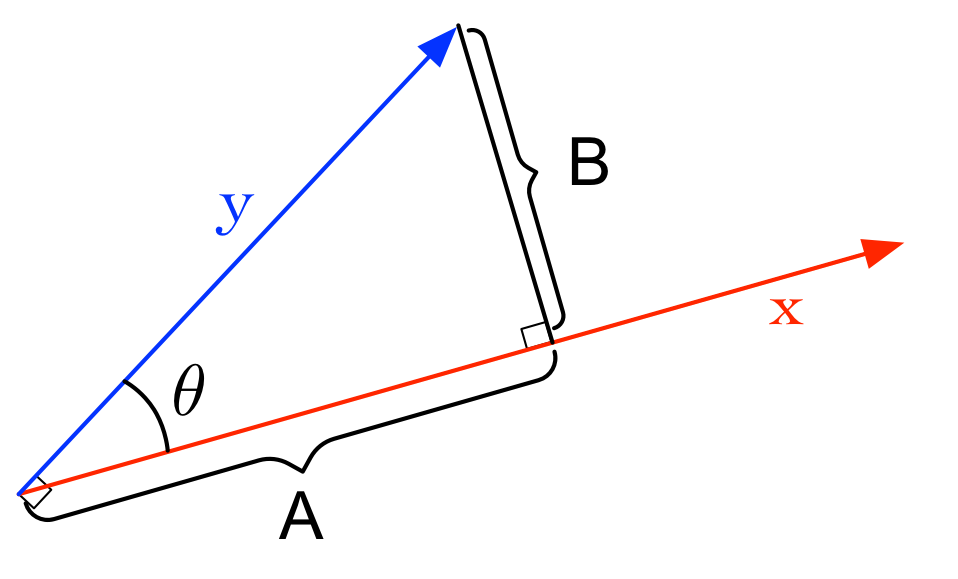
\includegraphics[scale=0.5]{cosine}
\label{fig:cosine}
\end{figure}

\noindent
Once we isolate cos(\(\theta\)) in (27) by dividing the Dot Product of \(x,y\) we then have a geometric interpretation of vector similarity or distance.
\begin{equation}
\begin{split}
    similarity = cos(\theta) &= \dfrac{x \cdot y}{||x||\,||y||} = \dfrac{\sum^n_{i=1} x_i y_i}{\sqrt{\sum^n_{i=1} x_i^2} \sqrt{\sum^n_{i=1} y_i^2}}
\end{split}
\end{equation}
\noindent
\begin{lemma}{2.10.3.1}\textbf{Law of Cosines}: To understand how we arrive at Cosine Similarity, we can understand the Law of Cosines, which given the triangle in Figure \ref{fig:cosine} with sides $y, B, and A$ is
\begin{equation}
\begin{split}
B^2 &= y^2 + A^2 - 2yA cos(\theta) \\
\end{split}
\end{equation}
\noindent
We can think of $B^2$ as 
\end{lemma}
Similarity ranges from, $-1$ meaning exactly opposite, $1$ meaning exactly the same, $0$ indicating orthogonality (decorrelation), and in-between values indicating intermediate similarity or dissimilarity.
\noindent
Note that since \(-1 \leq cos\theta \leq 1\), this is an alternative proof of the Cauchy-Schwartz inequality, by
\[\dfrac{|\langle x,y \rangle|}{||x|| \, ||y||} \leq 1\]
\end{corollary}
\end{definition}

%========================================================================================================================================

\begin{definition}{2.11} \textbf{Norm}: Given a vector \(x \in \mathbb{R}^n\) we define it's norm $||x||$ (distance to zero) as
\begin{equation}
\begin{split}
    ||x|| = x^T x = \sqrt{\sum^n_{i=1} x^2_i}
\end{split}
\end{equation}
\noindent
\begin{corollary}{2.11.1} \textbf{Properties of Norm} Let $V$ be a vector space, a norm is a function \(||\cdot||\) from $V$ to \(\mathbb{R}\) that satisfies the following conditions.
\begin{itemize}
    \item It is homogeneous. For all \(a \in \mathbb{R}\) and \(x \in V\) \[||ax|| = |a| \, ||x||.\]
    \item It satisfies the \textbf{triangle inequality} \[||x + u|| \leq ||x|| + ||y||.\]
    \noindent In particular, it is non-negative (set y = -x)
    \item \(||x|| = 0\) implies that x is the zero vector 0.
\end{itemize}
\end{corollary}
\end{definition}

%========================================================================================================================================

\begin{corollary}{2.11.2} \textbf{Distance} The distance between two vectors in a normed space with norm \(||\cdot||\) is
\[d(x,y) := ||x-y||.\]
\noindent
Inner-product spaces are normed spaces because we can define a valid norm using the inner product. The norm induced by an inner product is obtained by taking the square root of the inner product of the vector with itself,
\[||x||_{\langle \cdot, \cdot \rangle} := \sqrt{\langle x,x \rangle}\]
\noindent
The norm induced by an inner product is clearly homogeneous by linearity and symmetry of the inner product. \(||x||_{\langle \cdot, \cdot \rangle} = 0 \) implies \(x = 0\) because the inner product is positive semidefinite. We only need to establish that the triangle inequality holds to ensure that the inner-product is a valid norm as we do Definition 2.12.
\end{corollary}

%========================================================================================================================================

\begin{corollary}{2.11.3} \textbf{Interesting Example} If we take the vector space of smooth functions from [0,1] to \(\mathbb{R}\) that satisfy \(f(0) = 1 \textrm{and} f(1) = 1\) and define the inner product
\[\langle f, g \rangle = \int_0^1 f(t)g(t)dt,\]
\noindent
then integration by parts shows that the derivative (as a linear transformation) is anti-symmetric. You can see example in Section 2.7 of Strang.
\end{corollary}

%========================================================================================================================================

\begin{definition}{2.12} \textbf{Cauchy-Schwartz Inequality} In mathematics, the Cauchy-Schwarz inequality, is a useful inequality encountered in many different settings, such as \textbf{linear algebra, analysis, probability theory, vector algebra and other areas}. It is considered to be one of the most important inequalities in all of mathematics. For any two vectors, \(\forall x, y \in \mathbb{R}\) in a \textbf{inner product} space
\begin{equation}
\begin{split}
    |\langle x, y \rangle| &\leq ||x||_{\langle \cdot, \cdot \rangle} \, ||y||_{\langle \cdot, \cdot \rangle} \\
    |\langle x^T, y \rangle|| &\leq \sqrt{\langle x,x \rangle}\ \sqrt{\langle y,y \rangle}\ \\
    |\sum^n_{i=1} x_i y_i| &\leq \sqrt{\sum^n_{i=1} x_i^2}\ \sqrt{\sum^n_{i=1} y_i^2}\
\end{split}
\end{equation}
\noindent
Assume \(||x||_{\langle \cdot, \cdot \rangle} \neq 0\),
\begin{equation}
\begin{split}
    \langle x, y \rangle = -||x||_{\langle \cdot, \cdot \rangle}||y||_{\langle \cdot, \cdot \rangle} &\iff y = -\dfrac{||y||_{\langle \cdot, \cdot \rangle}}{||x||_{\langle \cdot, \cdot \rangle}}x. \\
    \langle x, y \rangle = ||x||_{\langle \cdot, \cdot \rangle}||y||_{\langle \cdot, \cdot \rangle} &\iff y = \dfrac{||y||_{\langle \cdot, \cdot \rangle}}{||x||_{\langle \cdot, \cdot \rangle}}x.
\end{split}
\end{equation}

\begin{proof}
If \(||x||_{\langle \cdot, \cdot \rangle} = 0\) then \(x=0\) because the inner product is positive semidefinite, which implies \(\langle x,y \rangle = 0\) and consequently that (19) holds with equality. The same is true if \(||y||_{\langle \cdot, \cdot \rangle} = 0\).
\noindent
Now assume that \(||x||_{\langle \cdot, \cdot \rangle} \neq 0\), \(||y||_{\langle \cdot, \cdot \rangle} \neq 0\), and \(t \in \mathbb{R}\). We construct a function,

\begin{equation}
\begin{split}
    p(t) &= ||ty - x||^2 \geq 0 \\
    &= (ty - x)(ty - x) \\
    &= ty \cdot ty - x \cdot ty - ty \cdot x + x \cdot x \\
    &= (y \cdot y)t^2 - 2(x\cdot y)t + x\cdot x \\
\end{split}
\end{equation}

\noindent
Set \(a = [(y \cdot y)], b = [2(x\cdot y)], c = [x\cdot x]\),
\begin{equation}
\begin{split}
    p(t) = at^2 - bt + c \geq 0
\end{split}
\end{equation}

%\noindent
%Since any quadratic \(ak^2+2bk+c\) takes its minimal value \(c-\dfrac{b^2}{a}\) when \(k = -\dfrac{b}{2a}\), and the inequality should hold for even this minimum value of the polynomial, so setting \(t=\dfrac{b}{2a}\)

\noindent
Set \(t = \dfrac{b}{2a}\)

\begin{equation}
\begin{split}
    p(\dfrac{b}{2a}) &= a\dfrac{b^2}{4a^2} - b\dfrac{b}{2a} + c \geq 0 \\
    &= \dfrac{b^2}{4a} - \dfrac{b^2}{2a} + c \geq 0 \\
    &= \dfrac{b^2}{4a} - \dfrac{2b^2}{4a} + c \geq 0 \\
    &= -\dfrac{b^2}{4a} + c \geq 0 \\
    c &\geq \dfrac{b^2}{4a} \\
    4ac &\geq b^2 \\
\end{split}
\end{equation}

\noindent
Substitute back into the equation for \(a, b, \textrm{and} \, c\).
\begin{equation}
\begin{split}
    4(||y||^2 \, ||x||^2) &\geq (2(x \cdot y))^2 \\
    4(||y||^2 \, ||x||^2) &\geq 4(x \cdot y)^2 \\
    ||y||^2 \, ||x||^2 &\geq (x \cdot y)^2 \\
    ||y|| \, ||x|| &\geq |x \cdot y|
\end{split}
\end{equation}

\noindent
Lastly, let's prove the equality again without assuming \(x=0\) or \(y=0\). Given \(x,y \in \mathbb{R}^n\) and \(c \in \mathbb{R}\), lets set \(x = cy\) giving us,

\begin{equation}
\begin{split}
    |x \cdot y| &= |cy\cdot y| \\
                &= |c| \, |y\cdot y| \\
                &= |c| \, ||y||^2 \\
                &= |c| \, ||y|| \, ||y|| \\
                &= ||cy|| \, ||y|| \\
                &= ||x|| \, ||y||
\end{split}
\end{equation}
\end{proof}
\end{definition}

\begin{definition}{2.13} \textbf{Triangle Inequality} \(||x+y|| \leq ||x||+||y||\)
\begin{proof}
\begin{equation}
\begin{split}
    ||x+y||^2 &= (x+y)\cdot(x+y) \\
    &= x\cdot(x+y)+y\cdot(x+y) \\
    &= x \cdot x + x \cdot y + y \cdot x + y \cdot y \\ 
    &= ||x||^2+2(x\cdot y)+||y||^2
\end{split}
\end{equation}

\noindent
And we know, by Cauchy-Schwartz inequality that,
\begin{equation}
\begin{split}
    x\cdot y \leq |x\cdot y| \leq ||x|| \, ||y||.
\end{split}
\end{equation}

\noindent
Thus establishing the inequality,

\begin{equation}
\begin{split}
    ||x+y||^2 &\leq ||x||^2 + 2||x||\,||y|| + ||y||^2 \\
\end{split}
\end{equation}

\noindent
And we see that the left hand side of (39) is a perfect square,

\begin{equation}
\begin{split}
    ||x+y||^2 &\leq (||x|| + ||y||)^2 \\
    ||x+y|| &\leq ||x||+||y|| \\
\end{split}
\end{equation}
\noindent
The triangle inequality is also “self-evident” when examining a sketch of $u$, $v$ and $u+v$.

\begin{figure}[h]
\caption{Illustration of Triangle Inequality}
\centering
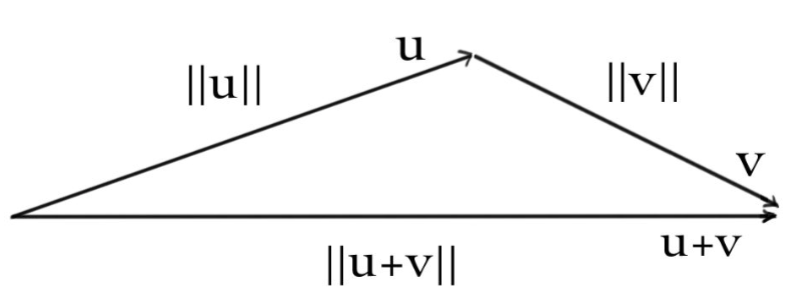
\includegraphics[scale=0.5]{triangle}
\label{fig:triequal}
\end{figure}

\end{proof}
\end{definition}

\begin{definition}{2.14} \textbf{Projection}: Given \(y,x \in \mathbb{R}^n\), the projection of $y$ onto the span of $x$ is given by,
\[P_{\langle x \rangle}(y) = \dfrac{x^T y}{||x||^2}x.\]

\begin{figure}[h]
\caption{Projection of $y$ onto span of $x$}
\centering
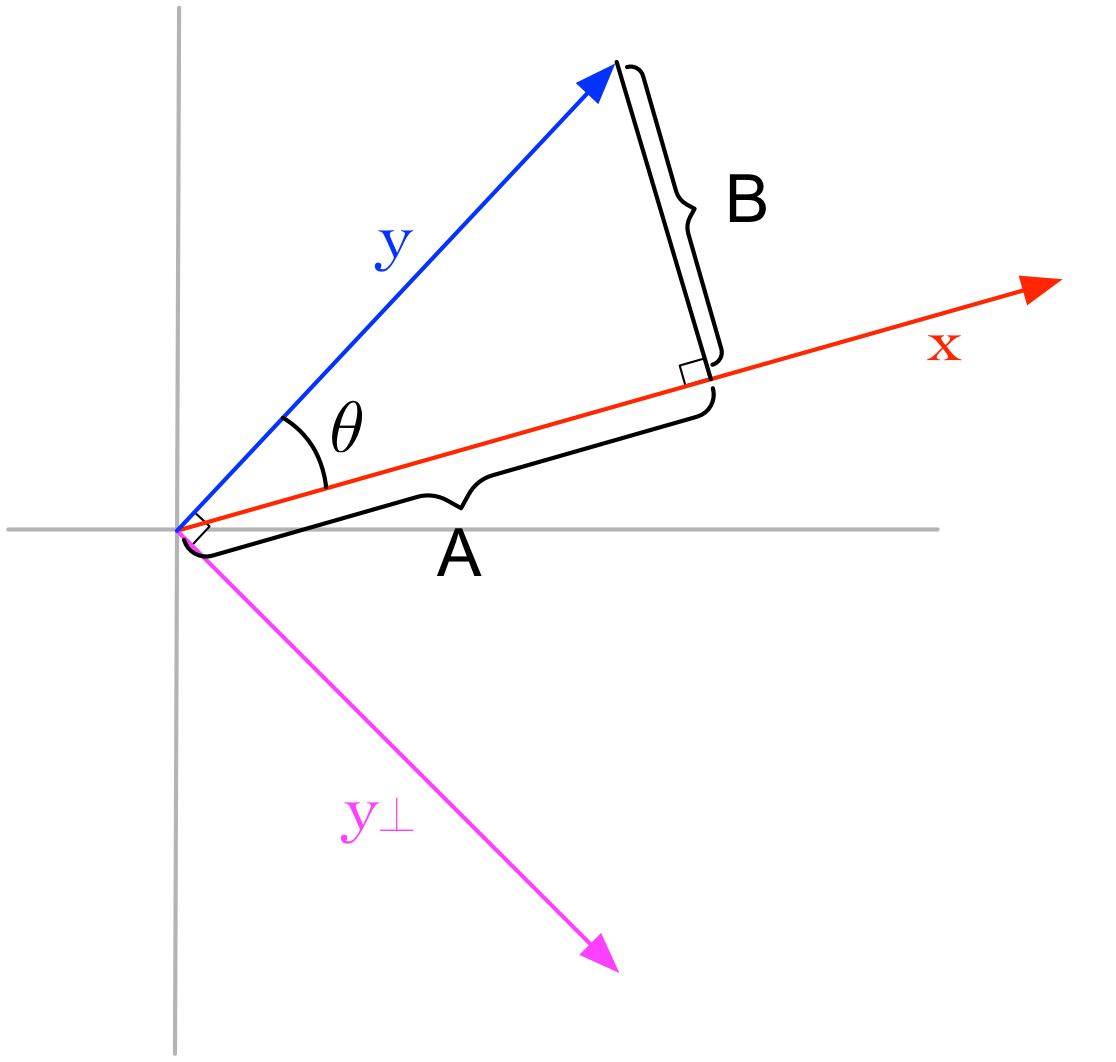
\includegraphics[scale=0.5]{projection}
\label{fig:prjctn2}
\end{figure}

\noindent
As can be seen from Figure \ref{fig:prjctn}:
\begin{itemize}
    \item A = 
\end{itemize}

\end{definition}

\begin{definition}{2.11.3} \textbf{Cosine Similarity}: Understanding the similarity of words that have been embedded into a vector can be gained by examining their cosine similarity. The cosine of two non zero vectors can be derived by using the Euclidean dot product formula.
\begin{equation}
\begin{split}
    x \cdot y &= ||x||\,||y||cos(\theta) \\
    cos(\theta) &= \dfrac{x \cdot y}{||x||\,||y||} \\
\end{split}
\end{equation}
\noindent
And, the similarity can then be understood by
\begin{equation}
\begin{split}
    similarity = cos(\theta) &= \dfrac{x \cdot y}{||x||\,||y||} = \dfrac{\sum^n_{i=1} x_i y_i}{\sqrt{\sum^n_{i=1} x_i^2} \sqrt{\sum^n_{i=1} y_i^2}}
\end{split}
\end{equation}
\noindent
Similarity ranges from, $-1$ meaning exactly opposite, $1$ meaning exactly the same, $0$ indicating orthogonality (decorrelation), and in-between values indicating intermediate similarity or dissimilarity.


\noindent
Note that since \(-1 \leq cos\theta \leq 1\), this is an alternative proof of the Cauchy-Schwartz inequality, by
\[\dfrac{|\langle x,y \rangle|}{||x|| \, ||y||} \leq 1\]
\end{definition}

\end{document}
